% This is file JFM2esam.tex
% first release v1.0, 20th October 1996
%       release v1.01, 29th October 1996
%       release v1.1, 25th June 1997
%       release v2.0, 27th July 2004
%       release v3.0, 16th July 2014
%       release v4.0, 15th June 2017
%   (based on JFMsampl.tex v1.3 for LaTeX2.09)
% Copyright (C) 1996, 1997, 2014, 2017 Cambridge University Press

\documentclass[12pt]{Style/RBM_P}
\usepackage{graphicx}
% \usepackage{epstopdf, epsfig}


\usepackage[utf8]{inputenc}
\usepackage[T1]{fontenc}
\usepackage{amsmath}
\usepackage{setspace}
\usepackage[a4paper, left=25mm, right=25mm, top=30mm, bottom=30mm]{geometry}

% \usepackage[square, comma, sort&compress, numbers]{natbib}
% \bibliographystyle{IEEEtran}

\usepackage[style=ieee]{biblatex}
\bibliography{reference/reference.bib}

\newtheorem{lemma}{Lemma}
\newtheorem{corollary}{Corollary}


\title{Title of RBM Research Proposal}


\begin{document}

% personal information
\newcommand{\StudentName}{Xiaoyun ZHONG}
\newcommand{\StudentID}{50013978}

\newcommand{\GroupProjectTitle}{A Metaverse Campus Community}
\newcommand{\ProjectManager}{Miaojun HUANG}
\newcommand{\ProjectSupervisor}{Miaojun HUANG}

\newcommand{\IndividualProjectTitle}{Multi-AI agent and multi-player perceptual interaction system and decision-making in Metaverse narrative game}

\newcommand{\Supervisor}{David Kei Man Yip}
\newcommand{\StuThrustHub}{CMA Thrust, Info Hub}


\begin{titlepage}
    \addcontentsline{toc}{section}{Title Page}
    \begin{center}
        \vspace*{1cm}

        \huge
        % \textbf{HKUST (GZ)}
        \vspace{0.5cm}

        \textbf{Thesis Proposal for MPhil Degree}

        \vspace{3cm}
        
        \begin{minipage}{0.8\textwidth}
            \Large
            \centering

            \begin{tabular}{l@{}ll}
                \textbf{Student Name}\vspace{0.5cm} &     & \wideunderline[16em]{\StudentName} \\
                \textbf{ID Number}\vspace{0.5cm} &     & \wideunderline[16em]{\StudentID} \\
                \textbf{Group Project}\vspace{0.5cm} &     & \wideunderline[16em]{{\GroupProjectTitle}} \\ 
                \textbf{Project Manager}\vspace{0.5cm} &     & \wideunderline[16em]{\ProjectManager} \\
                \textbf{Project Supervisor}\vspace{0.5cm} &     & \wideunderline[16em]{\ProjectSupervisor} \\
                \textbf{Individual Project}\vspace{0.5cm}&     & \wideunderline[16em]{{\IndividualProjectTitle}}  \\
                \textbf{Thesis Supervisor(s)}\vspace{0.5cm} &     & \wideunderline[16em]{{\Supervisor}}  \\
                \textbf{Student's Thrust \& Hub}\vspace{0.5cm} &     & \wideunderline[16em]{\StuThrustHub} \\
            \end{tabular}

        \end{minipage}

        \vfill

        \normalsize
        
        \newdateformat{monthyeardate}{%
        \THEMONTH/\THEYEAR}
        \renewcommand{\monthyeardate}{\ifcase \month \or 1\or 2\or 3\or %
        4\or 5 \or 6\or 7\or 8\or 9\or 10\or 11\or 12\fi/\number \year} \monthyeardate
        
        \text{The Hong Kong University of Science and Technology (Guangzhou)} 

    \end{center}
    \setcounter{page}{1} % set the page number to 1
\end{titlepage}
\spacing{1.5}

\maketitle


\begin{abstract}
\textbf{Abstract: } This file contains instructions for authors planning to submit \textit{Thesis Proposal for Red Bird Mphil}. These instructions were generated in {\LaTeX} according to the instruction provided by RBM, so the {\LaTeX} source file can be used as a template for submissions. The present paragraph appears in the \verb|abstract| environment. All papers should feature a single-paragraph abstract of no more than 250 words, which provides a summary of the main aims and results.
\end{abstract}

\section{How to submit to the \textbf{\textit{Thesis Proposal for Red Bird Mphil}}}
Authors must submit using the online submission and peer review system, ScholarOne Manuscripts (formerly Manuscript Central) at http://mc.manuscriptcentral.com/pla. If visiting the site for the first time, users must create a new account by clicking on `register here'. Once logged in, authors should click on the `Corresponding Author Centre', from which point a new manuscript can be submitted, with step-by-step instructions provided. Authors must at this stage specify the type of paper submitted: `original article' or `review' (see \S\ref{sec:filetypes} for more details). Once your submission is completed you will receive an email confirmation.
 

\section{Figures}
Figures should be as small as possible while displaying clearly all the information required, and with all lettering readable. Every effort should be taken to avoid figures that run over more than one page. There is no charge for colour figures. For review purposes figures should be embedded within the manuscript. Upon final acceptance, however, individual figure files will be required for production. These should be submitted in EPS or high-resolution TIFF format (1200 dpi for lines, 300 dpi for halftone, and 600 dpi for a mixture of lines and halftone). The minimum acceptable width of any line is 0.5pt. Each figure should be accompanied by a single caption, to appear beneath, and must be cited in the text. Figures should appear in the order in which they are first mentioned in the text and figure files must be named accordingly to assist the production process (and numbering of figures should continue through any appendices). For example see figures \ref{fig:ka} and \ref{fig:kd}. Failure to follow figure guidelines may result in a request for resupply and a subsequent delay in the production process.

\begin{figure}[h]
  \centering
  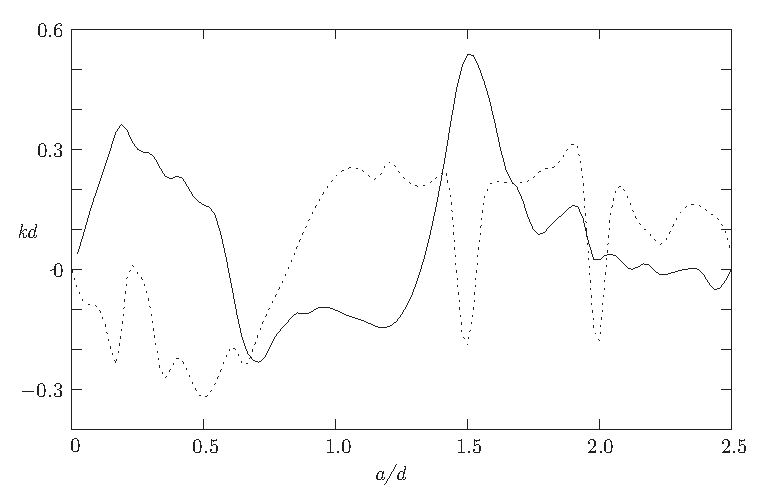
\includegraphics{image/trapped.eps}% Images in 100% size
  \caption{Trapped-mode wavenumbers, $kd$, plotted against $a/d$ for
    three ellipses:\protect\\%
    ---$\!$---,
    $b/a=1$; $\cdots$\,$\cdots$, $b/a=1.5$.}
\label{fig:ka}
\end{figure}

\begin{figure}
  \centering
  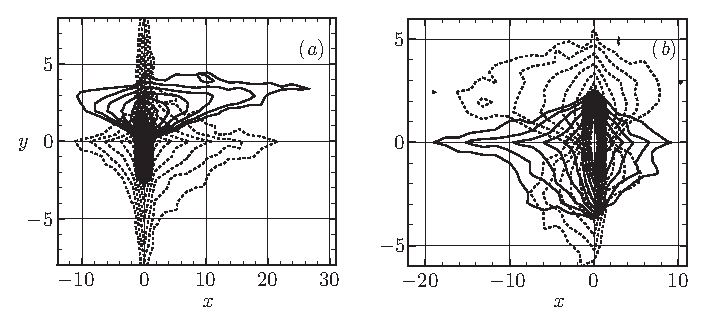
\includegraphics{image/modes}
  \caption{The features of the four possible modes corresponding to
  (\textit{a}) periodic\protect\\ and (\textit{b}) half-periodic solutions.}
\label{fig:kd}
\end{figure}

\subsection{Tables}
Tables, however small, must be numbered sequentially in the order in which they are mentioned in the text. The word \textit {table} is only capitalized at the start of a sentence. See table \ref{tab:kd} for an example.

\begin{table}
  
  \begin{center}
\def~{\hphantom{0}}
  \begin{tabular}{lccc}
      $a/d$  & $M=4$   &   $M=8$ & Callan \etal \\[3pt]
       0.1   & 1.56905 & ~~1.56~ & 1.56904\\
       0.3   & 1.50484 & ~~1.504 & 1.50484\\
       0.55  & 1.39128 & ~~1.391 & 1.39131\\
       0.7   & 1.32281 & ~10.322 & 1.32288\\
       0.913 & 1.34479 & 100.351 & 1.35185\\
  \end{tabular}
  \caption{Values of $kd$ at which trapped modes occur when $\rho(\theta)=a$}
  \label{tab:kd}
  \end{center}
\end{table}

\begin{plaintable}
  
  \begin{center}
\def~{\hphantom{0}}
  \begin{tabular}{lccc}
      $a/d$  & $M=4$   &   $M=8$ & Callan \etal \\[3pt]
       0.1   & 1.56905 & ~~1.56~ & 1.56904\\
       0.3   & 1.50484 & ~~1.504 & 1.50484\\
       0.55  & 1.39128 & ~~1.391 & 1.39131\\
       0.7   & 1.32281 & ~10.322 & 1.32288\\
       0.913 & 1.34479 & 100.351 & 1.35185\\
  \end{tabular}
  \caption{Values of $kd$ at which trapped modes occur when $\rho(\theta)=a$}
  \label{tab:kd}
  \end{center}
\end{plaintable}


\section{Notation and style}\label{notstyle}
Generally any queries concerning notation and journal style can be answered by viewing recent pages in the Journal. However, the following guide provides the key points to note. It is expected that Journal style will be followed, and authors should take care to define all variables or entities upon first use. Also note that footnotes are not normally accepted.

\subsection{Mathematical notation}
\subsubsection{Setting variables, functions, vectors, matrices etc}

\textbf{Italic font} should be used for denoting variables, with multiple-letter symbols avoided except in the case of dimensionless numbers.

\textbf{Upright Roman font} (or upright Greek where appropriate) should be used for:
\begin{itemize}
\item Operators: sin, log, d, $\Delta$, e etc.
\item Constants: i ($\sqrt{-1}$), $\upi$ (defined as \verb}\upi}), etc.
\item Functions: $\Ai$, $\Bi$ (Airy functions, defined as \verb|\Ai| and \verb|\Bi|), $\Real$ (real part, defined as \verb|\Real|), $\Imag$ (imaginary part, defined as \verb|\Imag|), etc.
\item Physical units: cm, s, etc
\item Abbreviations: c.c. (complex conjugate), h.o.t. (higher-order terms), DNS, etc.
\end{itemize}

\textbf{Bold italic font} (or bold sloping Greek) should be used for:

\begin{itemize}
\item  Vectors (with the centred dot for a scalar product also in bold): $\boldsymbol{i \cdot j}$
\end{itemize}

\textbf{Bold sloping sans serif font}, defined by the \verb|\mathsfbi| macro, should be used for:
\begin{itemize}
\item Tensors and matrices: $\mathsfbi{D}$
\end{itemize}

\textbf{Script font} (for example $\mathcal{G}$, $\mathcal{R}$) can be used as an alternative to italic when the same letter denotes a different quantity (use \verb|mathcal| in \LaTeX).

The product symbol ($\times$) should only be used to denote multiplication where an equation is broken over more than one line, to denote a cross product, or between numbers (the $\cdot$ symbol should not be used, except to denote a scalar product specifically).


\subsubsection{Other symbols}
A centred point should be used only for the scalar product of vectors.
Large numbers that are not scientific powers should not include commas, but have the
form 1600 or 16~000 or 160~000.
Use \textit{O} to denote `of the order of', not the \LaTeX\ $\mathcal{O}$.

\subsection{Equations}
Here are some equations for example.

\begin{equation}
  (\nabla^2+k^2)G_s=(\nabla^2+k^2)G_a=0
  \label{Helm}
\end{equation}

\begin{equation}
  -\frac{1}{2\upi} \int_0^{\infty} \gamma^{-1}[\mathrm exp(-k\gamma|y-\eta|)
   + \mathrm exp(-k\gamma(2d-y-\eta))] \cos k(x-\xi)t\:\mathrm{d} t,
   \qquad 0<y,\quad \eta<d,
\end{equation}

\begin{equation}
  \gamma(t) = \left\{
    \begin{array}{ll}
      -\mathrm{i}(1-t^2)^{1/2}, & t\le 1 \\[2pt]
      (t^2-1)^{1/2},         & t>1.
    \end{array} \right.
\end{equation}

\[
  -\frac{1}{2\upi}
   \pvi B(t)\frac{\cosh k\gamma(d-y)}{\gamma\sinh k\gamma d}
   \cos k(x-\xi)t\:\mathrm{d} t
\]

\begin{equation}
  G = -\frac{1}{4}\mathrm{i} (H_0(kr)+H_0(kr_1))
    - \frac{1}{\upi} \pvi\frac{\mathrm{e}^{-\kgd}}%
    {\gamma\sinh\kgd} \cosh k\gamma(d-y) \cosh k\gamma(d-\eta)
\end{equation}

Note that when equations are included in definitions, it may be suitable to render them in line, rather than in the equation environment: $\boldsymbol{n}_q=(-y^{\prime}(\theta),
x^{\prime}(\theta))/w(\theta)$.
Now $G_a=\squart Y_0(kr)+\Gat$ where
$r=\{[x(\theta)-x(\psi)]^2 + [y(\theta)-y(\psi)]^2\}^{1/2}$ and $\Gat$ is
regular as $kr\ttz$. However, any fractions displayed like this, other than $\thalf$ or $\squart$, must be written on the line, and not stacked (ie 1/3).
 
\begin{align}
  \ndq\left(\frac{1}{4} Y_0(kr)\right) & \sim 
    \frac{1}{4\upi w^3(\theta)}
    [x^{\prime\prime}(\theta)y^{\prime}(\theta)-
    y^{\prime\prime}(\theta)x^{\prime}(\theta)] \nonumber\\
  & =  \frac{1}{4\upi w^3(\theta)}
    [\rho^{\prime}(\theta)\rho^{\prime\prime}(\theta)
    - \rho^2(\theta)-2\rho^{\prime 2}(\theta)]
    \quad \mbox{as\ }\quad kr\ttz . \label{inteqpt}
\end{align}

\begin{equation}
  \frac{1}{2}\phi_i = \frac{\upi}{M} \sumjm\phi_j K_{ij}^a w_j,
  \qquad i=1,\,\ldots,\,M,
\end{equation}
where
\begin{equation}
  K_{ij}^a = 
      \begin{cases}
      \p G_a(\theta_i,\theta_j)/\p n_q, & i\neq j \\[2pt]
      \p\Gat(\theta_i,\theta_i)/\p n_q
      + [\rho_i^{\prime}\rho_i^{\prime\prime}-\rho_i^2-2\rho_i^{\prime 2}]
      / 4\upi w_i^3, & i=j.
      \end{cases}
\end{equation}


\refstepcounter{equation}
\[
  \rho_l = \lim_{\zeta \rightarrow Z^-_l(x)} \rho(x,\zeta), \quad
  \rho_{u} = \lim_{\zeta \rightarrow Z^{+}_u(x)} \rho(x,\zeta)
  \eqno{(\theequation{\mathit{a},\mathit{b}})}\label{eq35}
\]

\begin{equation}
  (\rho(x,\zeta),\phi_{\zeta\zeta}(x,\zeta))=(\rho_0,N_0)
  \quad \mbox{for}\quad Z_l(x) < \zeta < Z_u(x).
\end{equation}


\begin{subeqnarray}
  \tau_{ij} & = &
    (\overline{\overline{u}_i \overline{u}_j}
    - \overline{u}_i\overline{u}_j)
    + (\overline{\overline{u}_iu^{SGS}_j
    + u^{SGS}_i\overline{u}_j})
    + \overline{u^{SGS}_iu^{SGS}_j},\\[3pt]
  \tau^\theta_j & = &
    (\overline{\overline{u}_j\overline{\theta}}
    - \overline{u}_j \overline{\theta})
    + (\overline{\overline{u}_j\theta^{SGS}
    + u^{SGS}_j \overline{\theta}})
    + \overline{u^{SGS}_j\theta^{SGS}}.
\end{subeqnarray}

\begin{equation}
\setlength{\arraycolsep}{0pt}
\renewcommand{\arraystretch}{1.3}
\slsQ_C = \left[
\begin{array}{ccccc}
  -\omega^{-2}V'_w  &  -(\alpha^t\omega)^{-1}  &  0  &  0  &  0  \\
  \displaystyle
  \frac{\beta}{\alpha\omega^2}V'_w  &  0  &  0  &  0  &  \mathrm{i}\omega^{-1} \\
  \mathrm{i}\omega^{-1}  &  0  &  0  &  0  &  0  \\
  \displaystyle
  \mathrm{i} R^{-1}_{\delta}(\alpha^t+\omega^{-1}V''_w)  &  0
    & -(\mathrm{i}\alpha^tR_\delta)^{-1}  &  0  &  0  \\
  \displaystyle
  \frac{\mathrm{i}\beta}{\alpha\omega}R^{-1}_\delta V''_w  &  0  &  0
    &  0  & 0 \\
  (\mathrm{i}\alpha^t)^{-1}V'_w  &  (3R^{-1}_{\delta}+c^t(\mathrm{i}\alpha^t)^{-1})
    &  0  &  -(\alpha^t)^{-2}R^{-1}_{\delta}  &  0  \\
\end{array}  \right] .
\label{defQc}
\end{equation}

\begin{equation}
\etb^t = \skew2\hat{\etb}^t \exp [\mathrm{i} (\alpha^tx^t_1-\omega t)],
\end{equation}
where $\skew2\hat{\etb}^t=\boldsymbol{b}\exp (\mathrm{i}\gamma x^t_3)$. 
\begin{equation}
\mbox{Det}[\rho\omega^2\delta_{ps}-C^t_{pqrs}k^t_qk^t_r]=0,
\end{equation}

\begin{equation}
 \langle k^t_1,k^t_2,k^t_3\rangle = \langle
\alpha^t,0,\gamma\rangle  
\end{equation}

\begin{equation}
\boldsymbol{f}(\theta,\psi) = (g(\psi)\cos \theta,g(\psi) \sin \theta,f(\psi)).
\label{eq41}
\end{equation}

\begin{eqnarray}
f(\psi_1) = \frac{3b}{\upi[2(a+b \cos \psi_1)]^{{3}/{2}}}
  \int^{2\upi}_0 \frac{(\sin \psi_1 - \sin \psi)(a+b \cos \psi)^{1/2}}%
  {[1 - \cos (\psi_1 - \psi)](2+\alpha)^{1/2}}\mathrm{d}x,
\label{eq42}
\end{eqnarray}
\begin{eqnarray}
g(\psi_1) & = & \frac{3}{\upi[2(a+b \cos \psi_1)]^{{3}/{2}}}
  \int^{2\upi}_0 \left(\frac{a+b \cos \psi}{2+\alpha}\right)^{1/2}
  \left\{ \astrut f(\psi)[(\cos \psi_1 - b \beta_1)S + \beta_1P]
  \right. \nonumber\\
&& \mbox{}\times \frac{\sin \psi_1 - \sin \psi}{1-\cos(\psi_1 - \psi)}
  + g(\psi) \left[\left(2+\alpha - \frac{(\sin \psi_1 - \sin \psi)^2}
  {1- \cos (\psi - \psi_1)} - b^2 \gamma \right) S \right.\nonumber\\
&& \left.\left.\mbox{} + \left( b^2 \cos \psi_1\gamma -
  \frac{a}{b}\alpha \right) F(\frac{1}{2}\upi, \delta) - (2+\alpha)
  \cos\psi_1 E(\frac{1}{2}\upi, \delta)\right] \astrut\right\} \mathrm{d} \psi,
\label{eq43}
\end{eqnarray}
\begin{equation}
\alpha = \alpha(\psi,\psi_1) = \frac{b^2[1-\cos(\psi-\psi_1)]}%
  {(a+b\cos\psi) (a+b\cos\psi_1)},
  \quad
  \beta - \beta(\psi,\psi_1) = \frac{1-\cos(\psi-\psi_1)}{a+b\cos\psi}.
\end{equation}


\begin{equation}
\left. \begin{array}{l}
\displaystyle
H(0) = \frac{\epsilon \overline{C}_v}{\tilde{v}^{{1}/{2}}_T
(1- \beta)},\quad H'(0) = -1+\epsilon^{{2}/{3}} \overline{C}_u
+ \epsilon \skew5\hat{C}_u'; \\[16pt]
\displaystyle
H''(0) = \frac{\epsilon u^2_{\ast}}{\tilde{v}^{{1}/{2}}
_T u^2_P},\quad H' (\infty) = 0.
\end{array} \right\}
\end{equation}




\begin{lemma}

%\citet[][pp.~231--232]{Batchelor59}

Let $f(z)$ be a trial  function defined on $[0,1]$.  Let $\varLambda_1$ denote
the ground-state eigenvalue for $-\mathrm{d}^2g/\mathrm{d} z^2=\varLambda g$,
where $g$ must satisfy $\pm\mathrm{d} g/\mathrm{d} z+\alpha g=0$ at $z=0,1$
for some non-negative constant~$\alpha$.  Then for any $f$ that is not
identically zero we have
\begin{equation}
\frac{\displaystyle
  \alpha(f^2(0)+f^2(1)) + \int_0^1 \left(
  \frac{\mathrm{d} f}{\mathrm{d} z} \right)^2 \mathrm{d} z}%
  {\displaystyle \int_0^1 f^2\mathrm{d} z}
\ge \varLambda_1 \ge
\left( \frac{-\alpha+(\alpha^2+8\upi^2\alpha)^{1/2}}{4\upi} \right)^2.
\end{equation}
\end{lemma}



\begin{corollary}
Any non-zero trial function $f$ which satisfies the boundary condition
$f(0)=f(1)=0$ always satisfies
\begin{equation}
  \int_0^1 \left( \frac{\mathrm{d} f}{\mathrm{d} z} \right)^2 \mathrm{d} z.
\end{equation}
\end{corollary}


\section{Citations and references}

%All papers included in the References section must be cited in the article, and vice versa. Citations should be included as, for example ``It has been shown \citep{Rogallo81} that...'' (using the {\verb}\citep} command, part of the natbib package) ``recent work by \citet{Dennis85}...'' (using {\verb}\citet}).
The natbib package can be used to generate citation variations, as shown below. \cite{ngFederatedBayesianNetwork2022}

% \begin{itemize}
% \item \verb#\citet[pp. 2-4]{Galtier00}#:
% \citet[pp. 479-480]{Galtier00} 
% \item \verb#\citep[p. 6]{Worster92}#:
% \citep[p. 6]{Worster92}
% \item \verb#\citep[see][]{Koch83, Lee71, Linton92}#:
% \citep[see][]{Koch83, Lee71, Linton92}
% \item \verb#\citep[see][p. 18]{Martin80}#:
% \citep[see][p. 18]{Martin80}
% \item \verb#\citep{Brownell04,Brownell07,Ursell50,Wijngaarden68,Miller91}#:
% \citep{Brownell04,Brownell07,Ursell50,Wijngaarden68,Miller91}
% \end{itemize}

The References section can either be built from individual \verb#\bibitem# commands, or can be built using BibTex. The BibTex files used to generate the references in this document can be found in the zip file in the Instructions for Contributors section of the JPP website.

Where there are up to ten authors, all authors' names should be given in the reference list. Where there are more than ten authors, only the first name should appear, followed by et al.

Acknowledgements should be included at the end of the paper, before the References section or any appendicies, and should be a separate paragraph without a heading. Several anonymous individuals are thanked for contributions to these instructions.

\appendix

\section{}\label{appA}
This appendix contains sample equations in the JPP style. Please refer to the {\LaTeX} source file for examples of how to display such equations in your manuscript.



% susie put cite commands here, don't bother with citet etc just yet.

% \bibliographystyle{jpp}
% Note the spaces between the initials



% \bibliography{jpp-instructions}
\printbibliography
% \bibliography{reference/reference2}


\end{document}
